\documentclass[uplatex]{jsarticle}
\usepackage[dvipdfmx]{graphicx}
\usepackage[dvipdfmx]{hyperref}
\usepackage{pxjahyper}
\usepackage{amsmath}
\usepackage{amsfonts}

\title{EoSL-Chapt.2}

\author{鬼頭幸助}
\date{\today}
\begin{document}
\maketitle
\section{導入}
\subsection{教師あり学習の目的}

入力変数を使い、出力変数の値を推測すること。

\subsection{変数の呼称}
基本的には、「入力変数」と「出力変数」という言葉を使う。それぞれ以下のような別称がある。
\begin{itemize}
    \item 入力変数(inputs)

    独立変数(independent variables), 特徴量(features), 予測因子(predictors)

    \item 出力変数(outputs)

    従属変数(dependent valiables), 応答変数(responses)
\end{itemize}

\section{変数の種類と用語}
\subsection{変数の種類}
\begin{itemize}
  \item 量的な変数(quantitative)

  間隔尺度と比例尺度。距離の概念がある。

  例)患者の再発率

  \item 質的な変数(qualitative, categorical)

  名義尺度。順序の概念はない。

  例)手書き文字の分類

  \item 順序付きの質的な変数(orderd categorical)

  順序尺度。順序はあるが、間隔・距離の概念はない。

  例)あてはまらない・どちらでもない・あてはまる

\end{itemize}
量的な変数を推定する手法を「回帰」(regression),
質的な変数を推定する手法を「分類」(classification)と呼ぶ。

\subsection{質的データの扱い}
質的データは、数値で表現されることも多い。よく使われる方法は以下の通り。

\begin{itemize}

  \item 2値の場合

  0,1 や -1,1 で表す。理論的には、本当になんでもよい(距離が等しいとか考えなくていいので)。

  \item 3値以上の場合

  ダミー変数を用いる。

  $g_i \in G \to x_i = ( 0 \, \dots \ , 0, 1, 0, \dots ,0 ) \in \{0,1\}^{|G|}$

  冗長にも感じるが、対称性がうれしい(どの2点間も距離が等しい、など)。
  "one-hot encoding"とも呼ばれる。
\end{itemize}

\subsection{文字の使い方}
\begin{itemize}

  \item 入力変数

  一般論として書くとき:$X=[X_1, X_2, \dots , X_p]$(ただし、紙面の都合上横向きに書いているが、縦ベクトルである。)

  一組の観測値:$x_i$

  p変数・N個の観測値:
  \[
    \mathbf{X} = \left(
      \begin{array}{ccccc}
        x_{11} & \dots & x_{1j} & \dots & x_{1p} \\
        \vdots & \ddots & \vdots & \ & \vdots \\
        x_{i1} & \dots  & x_{ij} & \dots & x_{ip} \\
        \vdots & \ & \vdots & \ddots & \vdots \\
        x_{N1} & \dots & x_{Nj} & \dots & x_{Np}
      \end{array}
    \right)
  \]
  各行が一組の観測値、各列が一つの値に関する全観測値に相当。行は$x_i$, 列は$\mathbf{x}_j$と書く。
  一般論として書くときは、行数(縦方向の数)がパラメータ数$p$であったが、観測値の行列では縦横が逆であることに注意。
  \item 出力変数

  量的なら$Y$, 質的なら$G$というアルファベットを使う。小文字や添え字の使い方は同様。
  予測値は、上に ``^'' 付ける。$\hat{Y}$, $\hat{G}$など。読みは「ワイ・ハット」「ジー・ハット」
\end{itemize}

また、$Y$や$G$の推定値$\hat{Y}$や$\hat{G}$を求めるためには、大量の実際のデータが必要である。
観測値や、アンケートの回答、Amazonの購買履歴など。
これらのように、教師あり学習の予測値を算出する関係式を構築するための元データを、訓練データ(training data)と呼ぶ。

\section{最小二乗法と最近傍法}
教師あり学習における、最も基本的な2つの手法をざっくりと。
\begin{itemize}
  \item 最小二乗法による線形回帰
  \item 最近傍法
\end{itemize}


\subsection{線形モデルと最小二乗法}

入力変数$X^\mathrm{T}=[X_1, X_2, \dots , X_p]$から出力変数$Y$を推定したいとする。このとき、$X$と$Y$は
\[
  Y=\beta_0+\beta_1X_1+\dots+\beta_pX_p=X^\mathrm{T}\beta
\]
という関係であることを仮定し、訓練データから$\beta$の値として最適な値$\hat{\beta}$を求め、
\[
  \hat{Y}=\hat{\beta_0}+\hat{\beta_1}X_1+\dots+\hat{\beta_p}X_p=X^\mathrm{T}\hat{\beta}
\]
という式で$Y$の推定値$\hat{Y}$を求めるという手法。最適化は、残差二乗和(residual sum of squares, RSS)
\[
  \mathrm{RSS}(\beta)=\sum_{i=1}^{N}(y_i-x_i^\mathrm{T}\beta)^2
  =(\mathbf{y}-\mathbf{X}\beta)^\mathrm{T}(\mathbf{y}-\mathbf{X}\beta)
\]
を最小化することで行う。(2個目の式変形は以下の画像を参照。)
\begin{figure}[htb]
  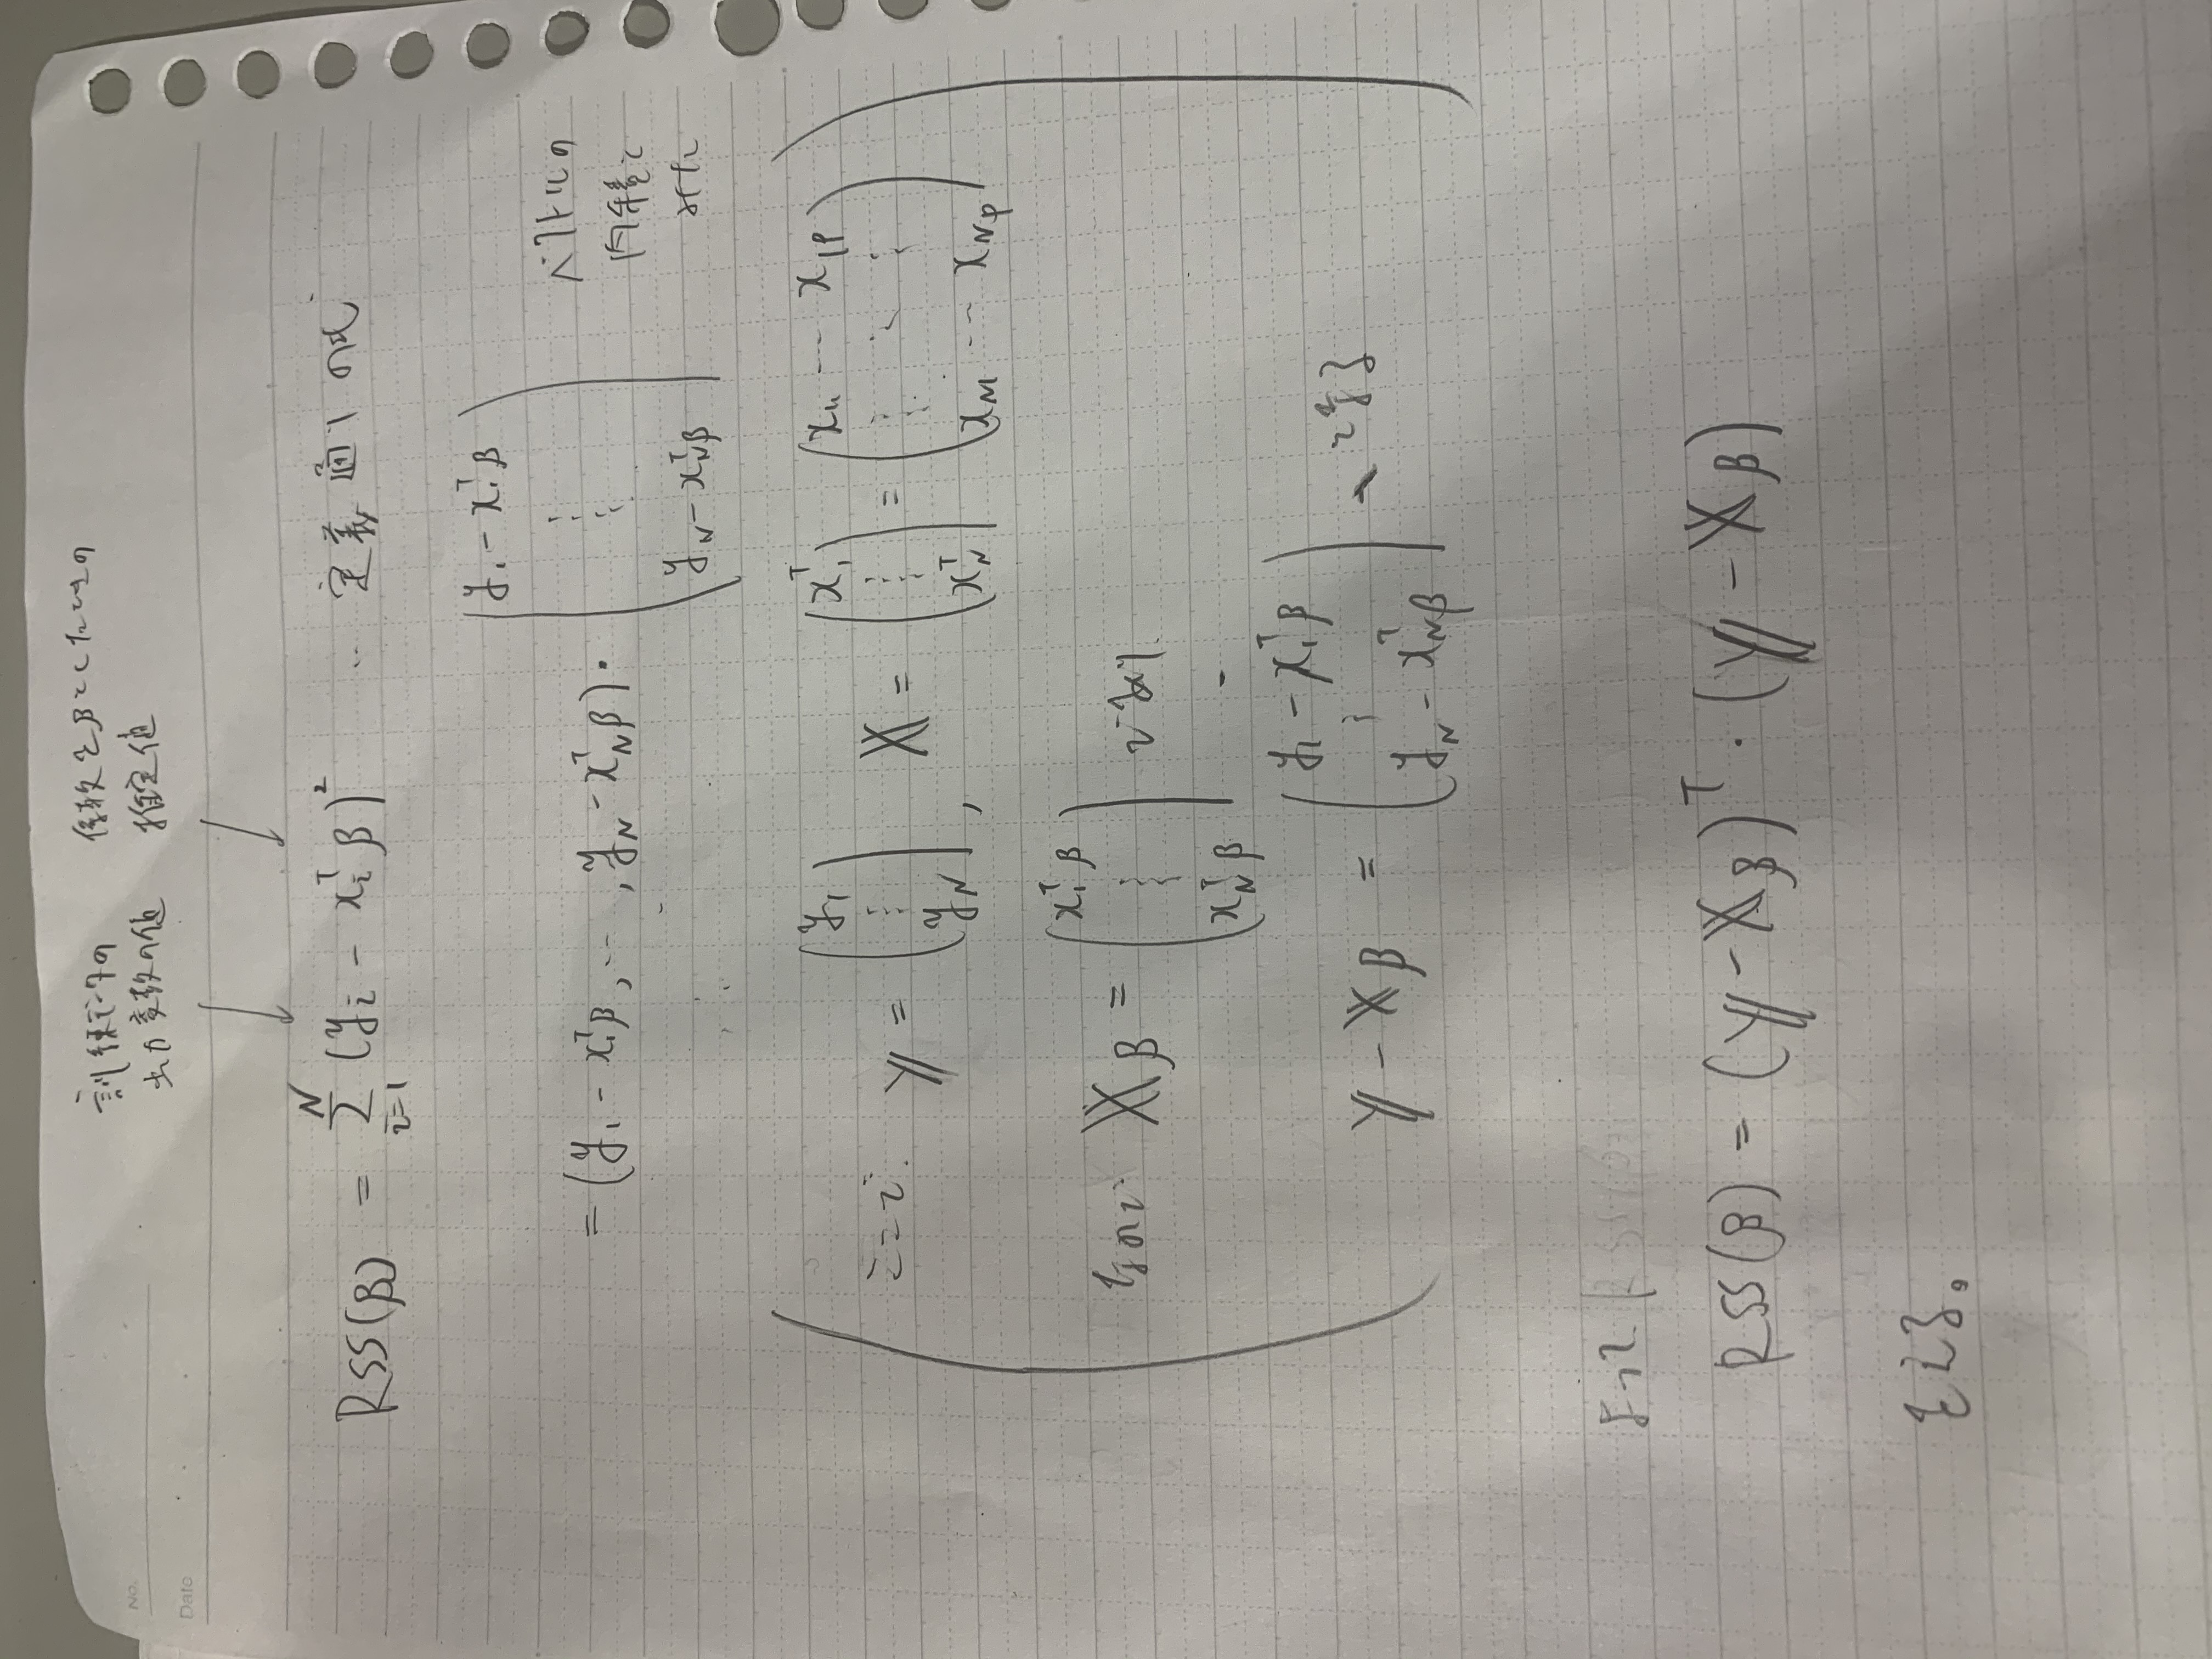
\includegraphics[width=100mm, angle=270]{fig-cal-1.jpg}
\end{figure}

これは、各$\beta_i$の二次式で、二乗の項の係数は非負なので最小値を持つ(まだ一意に定まるとは限らない)。微分して$=0$とすると、
\[
  \mathbf{X}^\mathrm{T}(\mathbf{y}-\mathbf{X}\beta)=0
\]
となる。(\href{https://qiita.com/AnchorBlues/items/8fe2483a3a72676eb96d}{行列・ベクトルの微分に関しては、こちらを参照。})(計算に関しては以下の画像を参照。)
\begin{figure}[htb]
  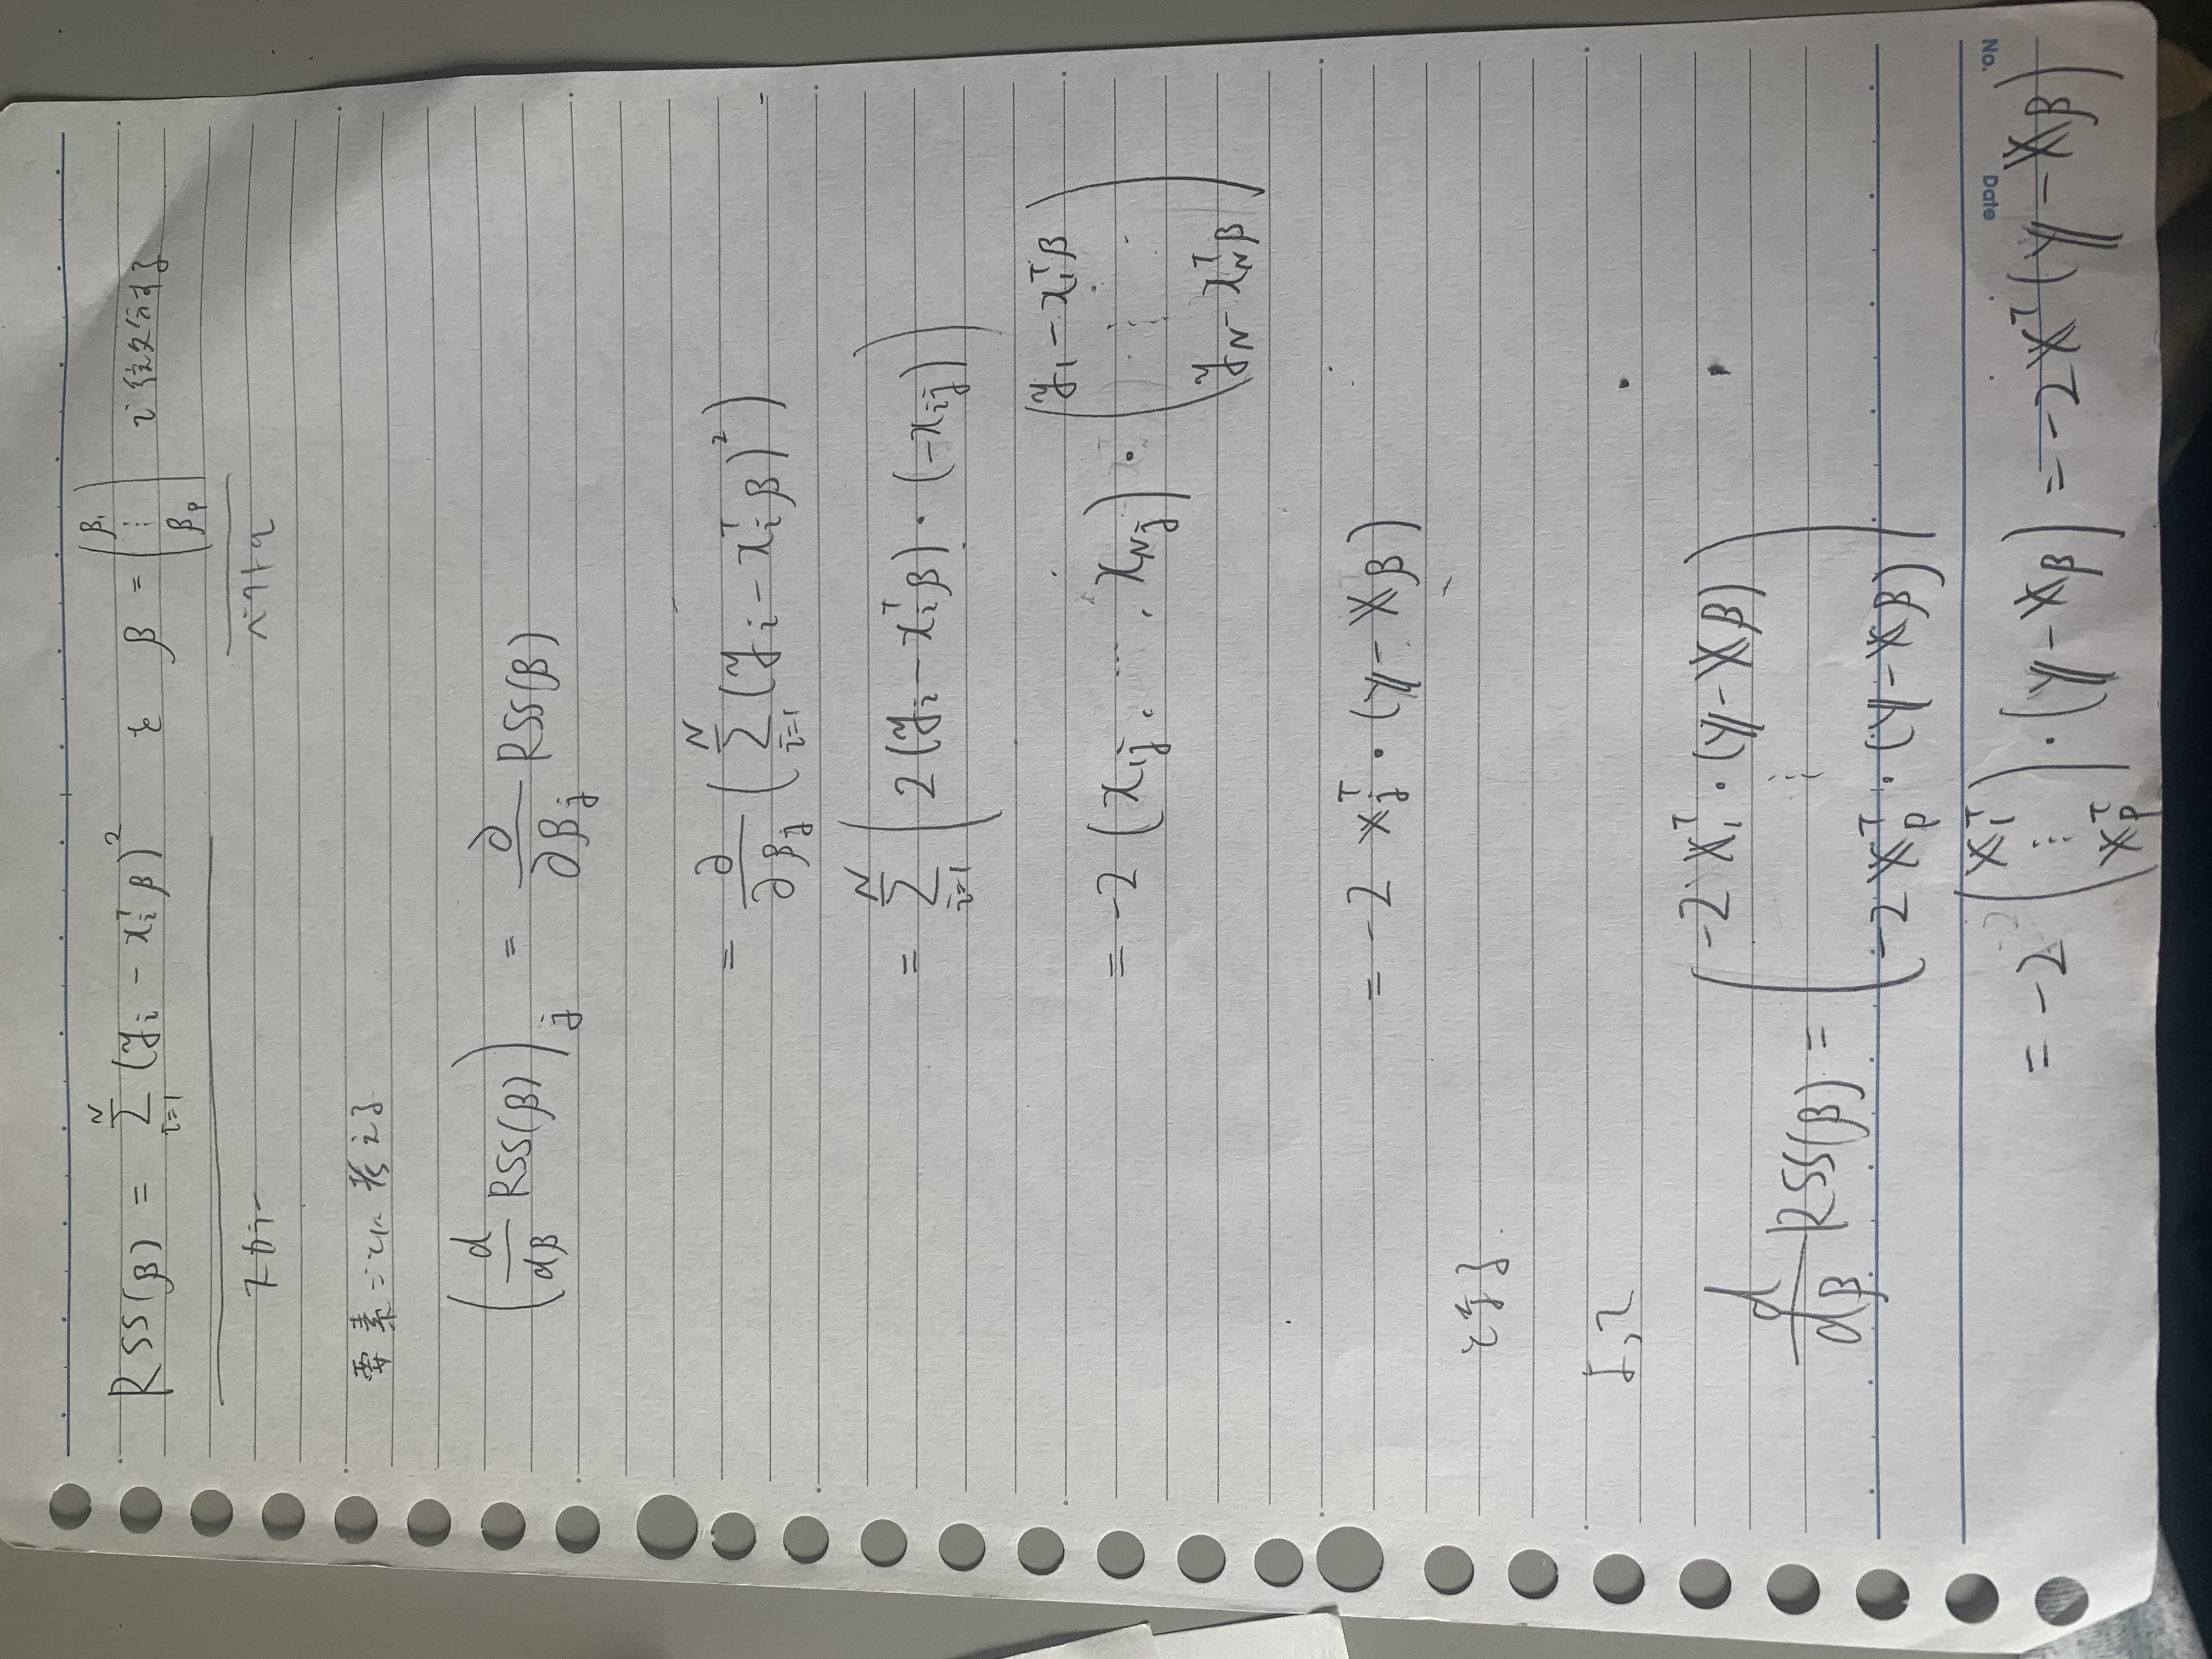
\includegraphics[width=100mm, angle=270]{fig-cal-2.jpg}
\end{figure}


これを解いて、
\[
  \hat{\beta}=(\mathbf{X}^\mathrm{T}\mathbf{X})^{-1}\mathbf{X}^\mathrm{T}\mathbf{y}
\]
となり一意に定まることが分かる。(ただし、$\mathbf{X}^\mathrm{T}\mathbf{X}$が正則の時のみ)

このように、入力変数と出力変数の関係式が線形関数であることを前提として行う回帰分析を線形回帰(linear regression)と呼ぶ。

線形回帰を分類問題に適用してみる。
平面$mathbb{R}^2$上に200個の点があり、そのうち100個には「ORANGE」、残りの100個には「BLUE」というラベルがついているとする。

この時、「ORANGE」→1, 「BLUE」→0 と数値化して、線形回帰をする。すると、平面内の各点に実数を割り当てるような回帰式
\[
  \hat{f} \colon \mathbb{R}^2 \to \mathbb{R}
\]
が得られる。よって、分類の推定として、
\[
  \hat{G}(x) =
  \begin{cases}
    \mbox{ORANGE} \quad \mathrm{if} \ \hat{f}(x) > 0.5 \\
    \mbox{BLUE}  \quad \mathrm{if} \ \hat{f}(x) \le 0.5
  \end{cases}
\]
という基準で分類している。つまり、境界線として、$\hat{f}(x)=0.5$という直線を採用しているのである。($\hat{f}$が線形関数なので、もちろん、境界線も線形になる。)

\begin{figure}[htb]
  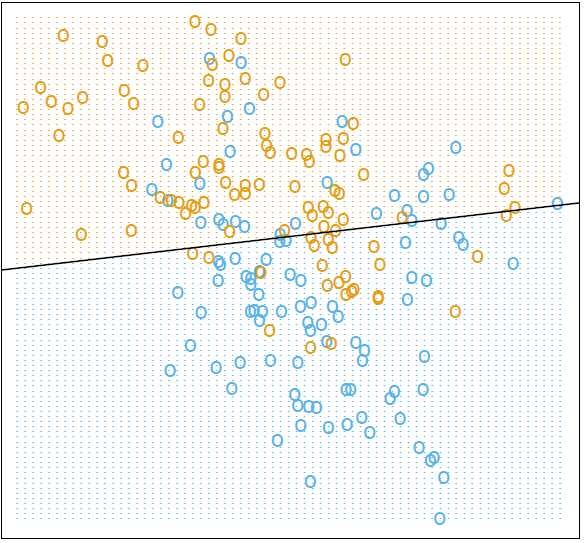
\includegraphics{fig2-1.png}
\end{figure}

この理論で、200個の訓練データをもとにORANGEとBLUEの分類を推定した結果が、画像の通り。

分類をミスっているものが多数ある。観測の誤差や外れ値の影響などで、このくらいは避けられないのか?もしくは、モデルが悪いのか(つまり、直線で分類できる、という仮説が良くないのか)?

ありえそうなシナリオは以下の通り。
\begin{itemize}

  \item 平均の異なる2つのガウス分布からそれぞれORANGEクラスとBLUEクラスが生成されている。
  →この時は、線形の境界が最適(Chapter4にて)

  \item それぞれのクラスが、いくつかのガウス分布からなる。
  →この時は、非線形の境界の方がいい。(今から見ていく)
\end{itemize}
\subsection{最近傍法}
「入力変数の値が近いなら、出力変数の値も近いのでは?」という仮説に基づいた手法。出力変数の推定値を、訓練データのうち、入力変数の値が近いものいくつかの出力変数の値の近いものの平均値として推定。
数式にすると、以下の様に推定。

まず、訓練データを
\[
  \mathcal{T}=\{ \ (x_i,y_i) \ | \ i=1,\dots,N\}
\]
として、点$x$の$k$近傍$N_k(x)$を、
\[
  N_k(x)=\{x_i\mbox{達のうち、}x\mbox{に近い方から}k\mbox{個}\}
\]
で定める。そのうえで、点$x$における出力変数$Y$の推定値$\hat{Y}(x)$を
\[
  \hat{Y}(x)=\frac{1}{k}\sum_{x_i \in N_k(x)}y_i
\]
で計算する。この手法をk-近傍法(k-nearest neighbor method, k-NN)という。

この手法を使うときは、kの個数をいくつにするのが良いかを考えたい。
→RSSは使えない。k=1とすればいつでも100%正解だが、明らかに過学習。
→kの値の「良さ」を評価する、異なる指標が必要になる。

\subsection{2つの手法の比較}
手法の良さの指標として、以下の二つが考えられる。
\begin{itemize}
  \item バイアス(bias)

  訓練データとのずれの大きさ。
  小さいほど、訓練データに適合している。

  \item バリアンス(variance)

  モデルの安定性。
  小さいほど、異なる訓練データを与えても、似たような予測値を返してくれる。
\end{itemize}

最小二乗法を用いた線形回帰と、最近傍法について、上記の2つの指標をざっくり評価すると、以下の通りになる。

\begin{table}[htb]
  \begin{tabular}{lllp{20em}}
    \ & variance & bias & \ \\
    線形モデル & low & high & きれいに分けられるけど、訓練データに合わないことが多い。\\
    最近傍法 & high & low & データにいくらでも合わせられるけど、分け方はぐっちゃぐちゃになることが多い。
  \end{tabular}
\end{table}


\section{統計的決定理論}

「教師あり学習」の理論を、一般的にまとめ、定式化する。

入力$X \in \mathcal{R}^p$, 出力$Y \in \mathcal{R}$が、$\mathrm{Pr}(X, Y)$という確率分布に従うと仮定。

実際の値と予測値のずれによるペナルティを規定する損失関数(loss function)を$L$と書く。すると、ペナルティの期待値を意味する、期待予測誤差(expected predictor error)が
\[
  \mathrm{EPE}(f)=\mathrm{E}_{X,Y}[L(Y,f(X))]
\]
で定まる。

これを最小化することが、「教師あり学習」の本質。とりあえず式変形。
\begin{eqnarray*}
  \mathrm{EPE}(f)&=&\int L(y, f(x)) Pr(dx, dy) \\
  &=&\int \int L(y,f(x)) Pr(y|x) dy Pr(x) dx \\
  &=& \mathrm{E} _X[E_{Y|X}[L(Y, f(X))|X]]
\end{eqnarray*}
となる。この式変形の要点は、$X,Y$全体での積分を、$X$の値を固定したときの$Y$での積分と、$X$での積分に分離できたこと。つまり、f(X)の値は、点ごとに最適化すればよい、とわかる。よって、ある確率分布に従う変数について、損失関数$L$によって誤差の評価を定めると、最も良い関係式として、
\[
  f(x)=\mathrm{argmin} _c E_{Y|X}[L(Y, f(X))|X]
\]
という式が得られる。

特に、損失関数として
\[
  L(Y, f(X)) = (Y-f(X))^2
\]
を取ることが多い。この時、関係式は
\[
  f(x) = \mathrm{E}[Y|X=x]
\]
と書けることが計算できる。

最近傍法の話を、この理論に合わせてみると、
\begin{itemize}
  \item 期待値を平均によって近似
  \item 条件付確率を近傍を取ることで近似
\end{itemize}
という、二つの近似をしていることが分かる。

また、線形モデルを仮定すると、
\[
  \mathrm{EPE}(f)=\mathrm{E}_X[(Y-X^\mathrm{T}\beta)^2]
\]
となる。これを微分して=0とすると、
\[
  \beta=(\mathrm{E}[XX^\mathrm{T}])^{-1}\mathrm{E}[XY]
\]
を得る。ここで、$X$を訓練データの行列に置き換えてあげれば、前に出した$\hat{\beta}$に一致する。

ちなみに、損失関数として、
\[
  L(Y, f(X)) = |Y-f(X)|
\]
を取ったとすると、
\[
  \hat{f}(x) = \mathrm{median}(Y|X=x)
\]
となる。

分類問題にこの理論を適用させてみる。
損失関数は、クラスの数を行と列とする、正方行列。よく使うのは、0-1損失関数
\[
\textbf{L} = \left(
    \begin{array}{cccc}
      0 & 1 & \dots & 1 \\
      1 & \ddots & \ddots & \vdots \\
      \vdots & \ddots & \ddots & 1 \\
      1 & \dots & 1 & 0
    \end{array}
  \right)
\]

i行j列の値は、本来$g_i$であるものを$g_j$と分類したときのペナルティ。
計算してあげると、

\[
  \hat{G}(x) = \mathrm{argmax}_g Pr(g|X=x)
\]

つまり、$x$というサンプルが観測されたときに、それがクラス$g$である確率が最も高いもの。
この分類の仕方をベイズ分類器(Bayes classifier)というらしい。

\section{高次元での局所的な手法}
「次元の呪い」(curse of dimentionality)というものがある。
次元が上がる(つまり、入力変数の数が増える)、想像以上に大変だよ、という話。

ここまでの話から、最近傍法の弱みは、サンプルが内包する誤差を学習しすぎてしまうことだった。であれば、サンプル数が十分多ければ、最近傍法でとてもよく推測できるのでは?
→高次元では、想像以上に大量のサンプルが必要になる、というお話。

線分、正方形、立方体の各辺を3等分して、辺縁にある部分の占める割合を計算すると分かりやすい。

空間内に適当な2点を取ったときの2点間の距離の期待値もどんどん増加する。

空間におけるサンプル数の密度=最近傍までの距離の期待値を保つには、p次元において$N^p$このサンプルが必要。めちゃくちゃ多い。

このように、次元が高まると、色々と困ることを「次元の呪い」という。

\section{統計モデル・教師あり学習・関数近似}
\subsection{誤差を組み込む話}
観測には、誤差がありうる。原因として考えられるのは
\begin{itemize}
  \item 未知の変数の存在
  \item 観測能力の限界
\end{itemize}
どちらにしても、なくすことはできないので、モデルも誤差があるものとして作る。誤差の組み込み方として最も一般的なのが、加法的(additive)なモデル。
\begin{eqnarray*}
  &Y=f(X)+\epsilon \\
  &f(X)=\mathrm{E}(Y|X=x), \ \mathrm{E}(\epsilon)=0, \ \epsilon \mbox{は} X \mbox{と独立。}
\end{eqnarray*}
ただし、分類問題では、加法的モデルは使わないことが多いとか。

\subsection{教師あり学習}
教師あり学習では、例から学ぶ。(learn from examples)
\begin{enumerate}
  \item $\hat{f}$を作る
  \item 各訓練データについて、誤差$y_i - \hat{f}(x_i)$を計算
  \item $\hat{f}$を修正する
\end{enumerate}

という繰り返し。(ちょっと何が言いたかった節なのか分からない。)

\subsection{関数近似}
入力変数や出力変数が値を取る空間はユークリッド空間と仮定。以下の式で推定を行う。
\begin{eqnarray*}
  Y&=&f_\theta(X) + \epsilon \\
  f_\theta(x) &=& \sum_{k=1}^Kh_k(x)\theta_k
\end{eqnarray*}

つまり、添え字づけられた関数の列$h_k$を基底とする線形結合であることを仮定する。(このような表記を線形基底展開(linear basis expansion)という。基底関数$h_k$としては、多項式や三角関数、シグモイドなどが使われたりする。

各パラメータ$\theta$を推定するには、線形モデルの時と同様に、RSSを使えばよい。

ただし、どうやら最小二乗法が効果を発揮でいない局面があるらしい。そういうときにも使える推定方法が、「最尤法」(maximum likelihood method)というもの。詳しくは後の章で解説されるが、ざっくりいうと、「手に入ったサンプルデータに対して、そのサンプルデータが取れる確率の最も高い分布を母集団のモデルの推定とする」という手法。

「尤」とは「もっともらしい」という意味で、サンプルから一番もっともらしい母集団を推定する、という意味合いがある模様。

\section{構造化された回帰モデル}
回帰関数としてどんな関数でもとって良い、としてしまうと、問題が発生する。すべての訓練データを通るような関数はいくらでも作れてしまうこと。

→このような関数は残差二乗和は0にするが、訓練データ以外の点をうまく推定できない。(過学習してしまっている状態)

この問題を解決する方法として考えられるのが、関数の候補に制限を加える方法。具体的な実装方法としては以下が考えられる。
\begin{itemize}
  \item 目的関数を最初からパラメータ入りの関数として表現し、パラメータを最適化する。
  \item 学習法に制限を加える。つまり、最適化の条件の中に、過学習を起こさせない計算を組み込む。
\end{itemize}
いずれの方法にしても、モデルの中に「複雑さ」(complexity)を表す数値を入れて、複雑さが高まると評価を下げるようにする、という方法がとられる。

\section{制限付きの推定法の分類}
前節でざっくりと話した、モデルに制限を加える方法。何種類かに分類できるので、ざっくりと紹介。ただし、この分類はmutually exclusiveではない。

\subsection{粗さに対するペナルティとベイズ法}
今までは、関数の「予測の良さ」の基準として残差二乗和を使ってきた。そこに、補正項を加える。式は以下の通り。
\[
  \mathrm{PRSS}(f;\lambda)=\mathrm{RSS}(f)+\lambda J(f)
\]
$J(f)$は関数$f$の粗さを要化する関数。つまり、急激に値が変化するような関数$f$に対しては、大きな値を取るような汎関数。よく使われるのは、立法平滑化スプライン(cubic smoothing spline, 和訳が正しいか不明)と呼ばれもの。以下の式で評価をする。
\[
  \mathrm{PRSS}(f;\lambda)=\sum_{i=1}^N(y_i-f(x_i))^2+\lambda\int(f''(x))^2dx
\]
$J(f)$の設定により、「粗さ」というものを具体的に規定し、$\lambda$の値によって、関数が訓練データに合致することと、粗くなりすぎないことのバランスを調整する。

上記のcubic smoothing splineにおいて、$\lambda=\infty$とすると、$J(f)=0$が必要になるので、線形モデルになる。

\subsection{カーネル法と局所回帰}
カーネル法は、残差二乗和の計算に際して、各項に重みを付ける方法である。
単純に言えば、近い訓練データを重視し、残差二乗和を計算する方法である。

まずは、カーネル関数(kernel function)$K_\lambda(x_0,x)$を一つとる。これは、点$x_0$での出力変数の値を推定するときの点$x$の値の持つ重みを表す。($\lambda$は、遠くと近くの重みのバランスを調整するパラメータ。)

そして、点$x_0$での値$f(x_0)$の推定値として、$f_{\hat{\theta}}(x_0)$を採用する。ただし、$f_{\theta}$は$\theta$でパラメータ表示された関数であり、パラメータの値$\hat{\theta}$は以下を最小化するようにとる。
\[
  RSS(f_\theta,x_0)=\sum_{i=1}^NK_\lambda(x_0,x_i)(y_i-f_\theta(x_i))^2
\]

具体例を見ておく。
\begin{itemize}
  \item $f_\theta=\theta_0$としたとき

  この時、上の式に代入して計算すると、
  \[
    \hat{y}=\hat{f}(x_0)=\theta_0=\frac{\sum_{i=1}^NK_\lambda(x_0,x_i)y_i}{\sum_{i=1}^NK_\lambda(x_0,x_i)}
  \]
  という重み付き平均であることが分かる。さらに、カーネル関数として、近いもの$k$個に$1$, それ以外に$0$を割り当てるような関数をつけば、これはk-近傍法に他ならない。
  \item $f_\theta=\theta_0+\theta_1x$としたとき

  この方法を「局所線形回帰モデル」というらしい。カーネル関数として定数関数を取れば、通常の線形回帰に他ならない。
\end{itemize}
\subsection{基底関数と辞書法}
数式の形は、先ほど見た線形基底展開と同じである。
\[
  f_\theta(x) = \sum_{k=1}^K\theta_kh_k(x)
\]

基底関数に候補は、事前に一覧で与えられていることが多く、「辞書法」(dictionary method)と呼ばれる。基底関数内にもパラメータが存在することもあり、そのような場合には、基底関数内のパラメータの推定も必要になる。

\section{モデル選択とバイアス・バリアンストレードオフ}
ここまで見てきたモデル内には、「複雑さ」を表す指標が組み込まれていた。
\begin{itemize}
  \item ペナルティ項の係数$\lambda$
  \item カーネル関数の広さを調整する変数$\lambda$
  \item 基底関数の数
\end{itemize}
これも学習の中で決定してあげる必要がある。

一般論として、複雑性の低すぎるモデルは、母集団をうまく表現できないので、訓練データ、テストデータ両方にうまく適合しない。

一方、複雑すぎるモデルは、訓練データが内包する誤差やずれ、偏りを学習しすぎてしまい、訓練データには非常によく適合するが、テストデータにはあまり適合しない。

このバランスを取ってあげる必要がある。

モデルの複雑さと、訓練データ、テストデータへの適合度はグラフのようになる。
\begin{figure}[htb]
  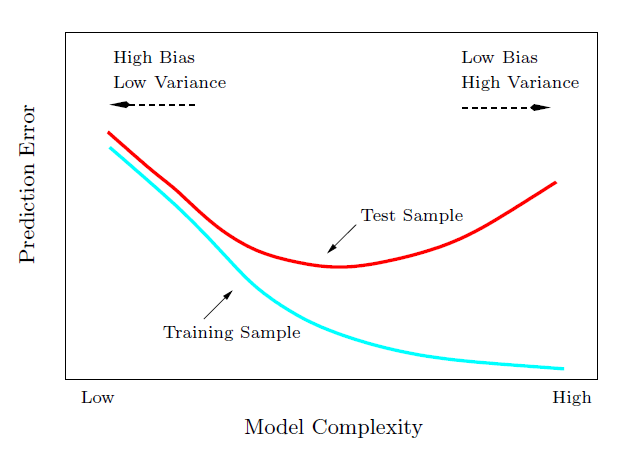
\includegraphics{fig2-11.png}
\end{figure}
\end{document}
